\documentclass{article}
\usepackage{graphicx}
\usepackage{hyperref}
\usepackage[a4paper, margin=1.25in]{geometry}
\usepackage{breakcites}
\usepackage{subcaption}
\usepackage{float}
\usepackage{textcomp}
\usepackage{amsmath}
\usepackage{textgreek}
\usepackage{authblk}
\usepackage{rotating}
\usepackage{booktabs}
\usepackage{longtable}
\usepackage{pdflscape}
\usepackage{subcaption}
\usepackage{lineno}
\usepackage[
  style=numeric,
  citestyle=numeric-comp,
  backend=biber,
  doi=true,
  natbib=true,
  sorting=none
]{biblatex}

\addbibresource{TextDataClimateShocks.bib}

\begin{document}
https://www.overleaf.com/project/5f918edd1afc380001feca0d
\title{Fine-scale Twitter Data Reveals Neighborhood Inequalities in Heat Wave Vulnerability}

%\author[1, *]{Matthew Cooper}
%\author[]{Jeremiah Osborne-Gowey}
%\author[]{Zheng Liu}
%\author[]{Jie Liu}
%\author[]{Portia Adade Williams}
%\author[]{Aaron Schwartz}
%\author[]{Patrick Baylis}

%\affil[1]{T.H. Chan School of Public Health, Harvard University}
%\affil[*]{Corresponding Author: mcooper@hsph.harvard.edu}

\maketitle

\begin{abstract}
Weather can affect people’s mood and well-being. Traditional studies exploring the effects of weather on mental health require significant resource investment (e.g., time, funding, execution).  Continuous in situ data streams from social media, newspapers, and other big data sources offer an opportunity to examine how people perceive and respond to environmental conditions. Recent work demonstrates that prevailing weather conditions can affect people’s sentiment as expressed on Twitter and other social media.  Studies to date however, have modeled the weather as having the same effect on sentiment across all locations and individuals (i.e., in aggregate).  In this study, we explore how weather affects individual expressed sentiment (via Twitter) across different weather gradients and locations. We analyzed the sentiment from a quarter of a billion geolocated Tweets from 2009 to 2019, using multiple measures of sentiment, overlaid with data about prevailing weather conditions, as well as local land cover, income levels, and demographic characteristics in the vicinity of Twitter users.  We find that weather affects people differently across a range of incomes, with people in higher income brackets generally happier with increasing temperature, while people in lower income brackets are less happy with increasing temperature.  This project extends existing research about the relationship between temperature and mood (sentiment) by examining how varying climatic conditions across different geographies and socio-economic groups are correlated with expressed sentiment. This project brings new insights into how humans perceive and respond to environmental shocks, with important implications for economics, policy and adaptation and resilience planning.

\end{abstract}

Keywords: Text Data, Environmental Shocks, Social Media Mining, Sentiment Analysis, Topic Modeling, Social Media, Public Opinion, Perception, Sentiment, Media, News, Twitter, Climate Change, Science Communication, Policy, Planning, Methods, Text Mining, Natural Language Processing, NLP, Latent Dirichlet Allocation, LDA, Political Ecology, Politics, Resilience, Adaptation, Suicide, Mortality, Morbidity, Self-harm, 

    
%Cite this new paper: https://doi.org/10.1016/S2542-5196(20)30251-5
% And: https://eos.org/articles/long-term-drought-harms-mental-health-in-rural-communities
\section{Introduction}

% Organize as follows:

% Heatwaves are known to worsen mental health
% AND mental health is strongly associated with income
% AND wealthier better able to cope with heatwaves 
% BUT we know little about the interaction between heatwaves, mental health and income
% THEREFORE: we did this really novel study.

This work builds on existing work by \citep{baylis_weather_2018}. 

%Intro Paragraph
Research has shown strong linkages between ambient environmental conditions and mental health, with extreme temperatures  frequently associated with poorer overall mental health. Individual's mental health is strongly associated with income with people in lower income levels frequently experiencing higher stress levels and less able to find help for coping with these stresses. Other research on how people cope with environmental temperature extremes indicate that wealthier are better able to cope with heatwaves, whether from traveling to cooler climes, accessing air conditioning, or other temperature ameliorating strategies that may require access to financial capital. Yet we know relatively little about the interaction between temperature, mental health and income. Furthermore, previous studies that did attempt to examine relationships between environmental extremes and health sometimes aggregated data at scales too coarse to examine whether income may be an ameliorating factor. This study examines the interactions between these three using relatively fine-scale, publicly available data. Our research expands on existing studies of temperature and sentiment - one measure of mental health - by examining finer-scale data and incorporating income data to examine correlations between temperature extremes and sentiment.

Human moods and mental states are important aspects of overall well-being and can be influenced by ambient, persistent and fluctuating environmental conditions. Climate change is accelerating the rate and variability around meteorological norms like the timing, magnitude, intensity and duration of precipitation events and air temperature minima and maxima \href{https://www.ipcc.ch/site/assets/uploads/2018/03/SREX-Chap3_FINAL-1.pdf}{(link)}. Previous work \citep{baylis_weather_2018} indicate important linkages between human mood and meterological conditions. Previous analyses of the effects of weather on mood (as expressed in sentiment of text-based message), however, were constructed at the aggregated city/day level and did not account for differences in socio-economic status which may affect access to resources (e.g., air conditioning) that can offset the effects of exposure to temperature extremes. Here, we build on these previous studies by examining the hourly effects of weather on human sentiment, an expression of mood, exploring geographic and economic heterogeneity at a finer-scale resolution than previous studies.  


\section{Background}
\subsection{Temperature and Mental Health}
% Heatwaves are known to worsen mental health



https://doi.org/10.1016/j.puhe.2018.06.008 (review study - will have more to cite)
https://www.nature.com/articles/s41558-018-0222-x
https://ehp.niehs.nih.gov/doi/full/10.1289/ehp.11339
https://ijmhs.biomedcentral.com/articles/10.1186/s13033-018-0210-6
https://www.nature.com/articles/s41558-018-0102-4/
https://doi.org/10.1016/j.jhealeco.2019.102240

[ADD SUICIDE DATA TO HEALTH SECTION?]
https://www.psychologytoday.com/us/blog/greening-the-media/201809/global-warming-and-suicide

\subsection{Mental Health and Income}
% AND mental health is strongly associated with income
% 1)Childhood 2)adulthood 3)gender
% Perceived income level

The relationship between income, socioeconomic status (SES), well-being and mental health is one of the strongest established patterns in psycho-social literature (cite: Easterlin 1973, Holzer et al. 1986, Perry 1996, Ng et al. 2014). Much of the research into these patterns focuses on the inequalities and distribution of the effects on individual well-being. Subsequent work on mental health outcomes, one measure of well-being, have established strong associations between SES, income and mental health with the most and least privileged most commonly associated with the best and worse mental health experiences and outcomes, respectively (cites: Stevenson and Wolfers 2008, Ng et al. 2014). 

For example, results from a cross-sectional comparative study of socioeconomic factors and use of mental health services by people living in Ontario, Canada and the United States, indicate clear disparities in use of mental health services between those with the highest income levels and lowest mental health morbidity and those with the lowest income levels and highest mental health morbidity - those with higher incomes tended to have lower mental health morbidity issues while utilizing mental health services more than those with lower incomes and higher mental health issues (cite Katz et al. 1997). 

Results from a systematic review of the literature on associations between social inequalities and mental health disorders indicate a clear and prevailing link between  one or more indicators of less social privilege and higher prevalence of mental health disorders (cite Fryers et al. 2003), with low income one of the most consistent markers of and associations with increases in common mental health disorders. Collectively, results from the income and mental health literature indicate that socially disadvantaged populations experience significantly more frequent common mental health disorders. Scholars use mental health disparities to indicate the disproportionate amount of mental health disorders among persons of low SES\citep{RN1292}

The established association between poverty and mental health revealed that that income distribution may have a significant influence upon mental health over and above the effect of poverty \citep{HANANDITA201459}.Poverty has been identified as one of the major risk factors in mental health. For instance, some systematic reviews have shown that socioeconomically disadvantaged children and adolescents were 2-3 times more likely to have mental health problems than others\citep{REISS201324}, while the household increases in financial resources are generally associated with an overall reduction of mental health problems\citep{2015Does}. Others have argued that increases in SES can serve as a buffer against the negative impacts of difficult life experiences on mental health, particularly for individuals already under substantive mental stress (cite Kawachi and Berkman 2001). Thus, SES and income are associated with mental health improvements in SES and income can serve to decrease menta the 

 
 Several reason could explain why poverty may effect mental health. 1) the “social causation hypothesis” which suggests that stress or deprivation or decreasing the likelihood of people getting treatment may lead to poor mental health\citep{mills2015}, while social capital could reduce the likelihood of living in poverty and reduces the risk of mental disorders such as depressive symptoms and suicidal tendencies\citep{RN1291}. 2) negative life events in a person’s life such as job loss are also associated with the risks of poverty\citep{RN1293} and mental health\citep{TAMPUBOLON201420}, and the causal inferences on the effect of poverty and mental health had also been made in several studies. For example, Tampubolon and Hanandita\citep{TAMPUBOLON201420} find that individual social capital is positively associated with mental health while adverse events were negatively associated; Chang.et.al \citep{RN1291} find that subjective and objective poverty is significantly associated with a higher risk of adverse life events, less social support and mental distress. Negative life events and social support in serial mediate the relationship between subjective poverty and mental health.

For children, poverty and poor maternal mental health often co-exist and are two of the risk factors for child development\citep{LUND20111502}, and maternal mental health is significantly associated with child general psychopathology\citep{ RN1289}. Researchers also find that transition into poverty increased children’s socioemotional behavior problems and maternal psychological distress \citep{WICKHAM2017e141}.

In general, the relationship between mental health and income level is well established. In the study, we explore whether income level would influence the link between weather and the sentiment in Twitter-posed text.

https://jamanetwork.com/journals/jamapsychiatry/fullarticle/211213
https://doi.org/10.1002/9781118410868.wbehibs570
https://www.sciencedirect.com/science/article/abs/pii/S027795362030527X
https://www.sciencedirect.com/science/article/pii/S2468266717300117
https://doi.org/10.1016/S2468-2667(17)30011-7
https://link.springer.com/article/10.1007/s00127-017-1370-4
Maybe this: https://journals.plos.org/plosone/article?id=10.1371/journal.pone.0116820
https://www.sciencedirect.com/science/article/abs/pii/S0143622814002537
also this: https://www.sciencedirect.com/science/article/abs/pii/S0140673614614604

\subsection{Income and Temperature}
% AND wealthier better able to cope with heatwaves 
https://www.nature.com/articles/nclimate3253
https://www.sciencedirect.com/science/article/abs/pii/S0378778818321327
https://www.mdpi.com/2225-1154/8/1/12/htm

NOT CLEAR: https://doi.org/10.1016/j.jhealeco.2019.102240 and https://www.nature.com/articles/s41558-018-0222-x find little evidence of adaptation

% BUT we know little about the interaction between heatwaves, mental health and income


% THEREFORE: we did this really novel study.
https://www.nature.com/articles/s41598-017-12961-9

%OTHER LEFTOVER TEXT TO MAYBE BRING IN LATER



Meteorological conditions can impact human physical (cite) and emotional states (cite). Emotional states and well-being are associated with physiological functioning and mental acuity which can affect social relationships, workplace productivity (cite) and health risks (cite). People that are more reliant on 1) livelihoods which require them to be outdoors (e.g., farming, agriculture, logging, etc.), 2) living and working in places where they are exposed to environmental minima and maxima, or 3) with prolonged exposure to ambient meteorological extremes are particularly vulnerable to changes in environmental exposure \citep{frimpong_heat_2017} and associated health risks (cite). Exposure to extreme environmental conditions can also have implications for workplace productivity and livelihoods \cite{kjellstrom_impact_2016}. For example, Nigerian maize farmers experience significant declines in productivity (2-8percent per degree above 17degC) along with substantive increases in health impacts including dehydration, muscle cramps, headaches and dizziness, heat exhaustion, sun stroke, and even death \cite{sadiq_impact_2019}. Other research indicates farm health and labor productivity were compromised under extreme heat and cold events in the Nepali Food Bowl region \cite{budhathoki_socio-economic_2019}. Similarly, Oregon farmers reported health impacts of working in both hot and cold conditions but the negative impacts were attenuated relative to the high heat situations \cite{bethel_heat-related_2014}. Other research found occupational injuries in Thailand increased with increasing heat exposure and occupational heat stress \cite{tawatsupa_association_2013}. Heat exposure risks are also a key factor in urban areas with particular attention needed for how the impacts of changing climate play out in health inequality \cite{friel_urban_2011}. 

Current estimates place annual workplace productivity losses due to heat exposure at 15-20percent with that rate potentially doubling by 2050 \cite{kjellstrom_heat_2016}. Projected increases in future ambient temperature suggest serious short- and long-term potential health consequences from exposure to heat stress (cite) with some estimates putting potential productivity losses at several percentage points by 2030 \cite{kjellstrom_heat_2016}, with middle- and low-income countries particularly vulnerable as they are often more reliant on physical work for their livelihoods. 

The level of changes in weather influences people’s mental health and patterns of emotions expressed. A study by Sun et al. 2018 \href{file:///Users/portia/Downloads/ijerph-16-00086-v2 20(1).pdf.}{(Portia has this PDF?)} demonstrates varied relationships between haze and negative emotions of the public under different seasons of the year. Being sad or happy influences one's style and value of reasoning. Time of day, season, location, and climate allow aggregate prediction of sentiments \cite{hannak_tweetin_2012} \href{https://www.ccs.neu.edu/~amislove/publications/Weather-ICWSM.pdf}{(link to PDF)} while positive affect from an evaluative statement enhances potential responses \cite{clore_how_2007} \href{https://www.ncbi.nlm.nih.gov/pmc/articles/PMC2483304/pdf/nihms40349.pdf}{(link to PDF)}. For instance, changes in temperature affects people’s response about weather. Depending on a reference temperature for an  area and time of year, people are more likely to comment on unusual weather for a particular place and time than on the same weather considered typical in another place \cite{moore_rapidly_2019}.

Although climate change is an international phenomenon experienced in every country, its discussions vary from country to country. According to Vu and others \cite{vu_nationalizing_2019}, a country’s climate severity, economic status and governance determine variations in its media discussions. For example, Park and others \cite{park_mood_2013} \href{https://pdfs.semanticscholar.org/b282/feb759e57530b115dcc4bb080f96598a5246.pdf}{(link)} demonstrated that many people living in a state with higher mean temperature express more positive emotions on Twitter than those living in colder states in the US. Schmidt and others \cite{schmidt_media_2013} posit that climate severity and environmental factors related to carbon dependency influences the amount of coverage climate change receives in the media in countries like USA, Australia and Germany. Studies comparing how different countries portray climate change have been widely conducted in USA, UK, France and the Netherlands \cite{vu_nationalizing_2019}. Such comparisons are mainly between developed countries with developing countries outside the focus.  Schafer and O’Neil \cite{schafer_what_2013} advance the need for academic scholars to investigate transnational contexts within climate communication. Wealthier countries with comparatively higher GDP are likely to frame climate change as a political issue as financial resources exist for exploring research on climate change. Conversely, coverage of climate change news from poorer developing countries focus mainly on international relations. Thus, the effects of national macro economic variables that affects a country’s sociopolitical and economic development such as GDP reflects a country’s governance system in media coverage \cite{vu_what_2018}. Cultural theorists assert that, understanding such differential variations depicts how different entities interpret danger and respond to risk \cite{tansey_cultural_1999}. Inclusion of developing countries in scientific research provides an avenue for international support to such countries in responding to the effects of climate change.Yet studies attempting to explain cross-national variation in climate change public opinion is limited \cite{knight_public_2016}.

Public debates on the current consequences of climate change are discussed in both scientific and non-scientific mediums. People can express their emotional states and feelings - sentiment - through physical, vocal and written expressions on mediums including newspapers, scientific articles, blogs and other online social media platforms. Twitter is one of the more popular social media platforms where people express their sentiments about any number of topics. Public posts on Twitter - called tweets - are widely available for public consumption and research, and offer a glimpse into collective social state. For example, text posted to these platforms can be used to gauge the public mood, assess opinions, measure brand affinity and for emergency planning and disaster response (cites). Sentiment is frequently employed as a correlate of emotional state or mood (cites). Weather events focus public attention in different ways of expression (cites). These data offer a unique opportunity to analyze how people express and respond to events in people's daily lives, including their exposure to ambient environmental conditions.



Here, we report on associations between meteorological conditions and expressed sentiment of public posts on Twitter from the United States of America (USA) between 2009 and 2019. This work builds on research from Baylis and others \cite{baylis_weather_2018} on weather impacts on expressed sentiment. In particular, we extend this work by including the temperature effects on sentiment in multiple regions across the USA while drawing in various climatic variables and socio-demographic data. In this research, we explore two primary questions. First, to what extent are amibent environmental conditions correlated with changes in expressed sentiment? Second, is this effect moderated by wealth? and local land cover conditions?

Building on previous findings from Baylis and others, we hypothesize that local ambient environmental conditions have a strong connection how people are feeling as expressed in the sentiment of text messages posted on Twitter [H1]. Second, we hypothesize that the weather-sentiment link will be stronger in low-income areas. That is to say, people in lower income areas will be have lower sentiment scores than those in wealthier areas. [H2].

\section{Results}
We examined the relationship between the sentiment expressed in tweets and the prevailing Wet Bulb Globe Temperature (WBGT), an indicator of heat stress that accounts for temperature, humidity, wind speed, and solar radiation.  We then explored how the racial and income characteristics of neighborhoods moderate the relationship between WBGT and sentiment.  Finally, we show how twitter sentiment is an important overall indicator of mental health by assessing the relationship between daily sentiment at the county level and the prevalence of crime and suicide. 

and sentiment, first examining the overall relationship, and then exploring heterogeneities based on neighborhood income per capita and race.

\begin{figure}[H]
  \centering
  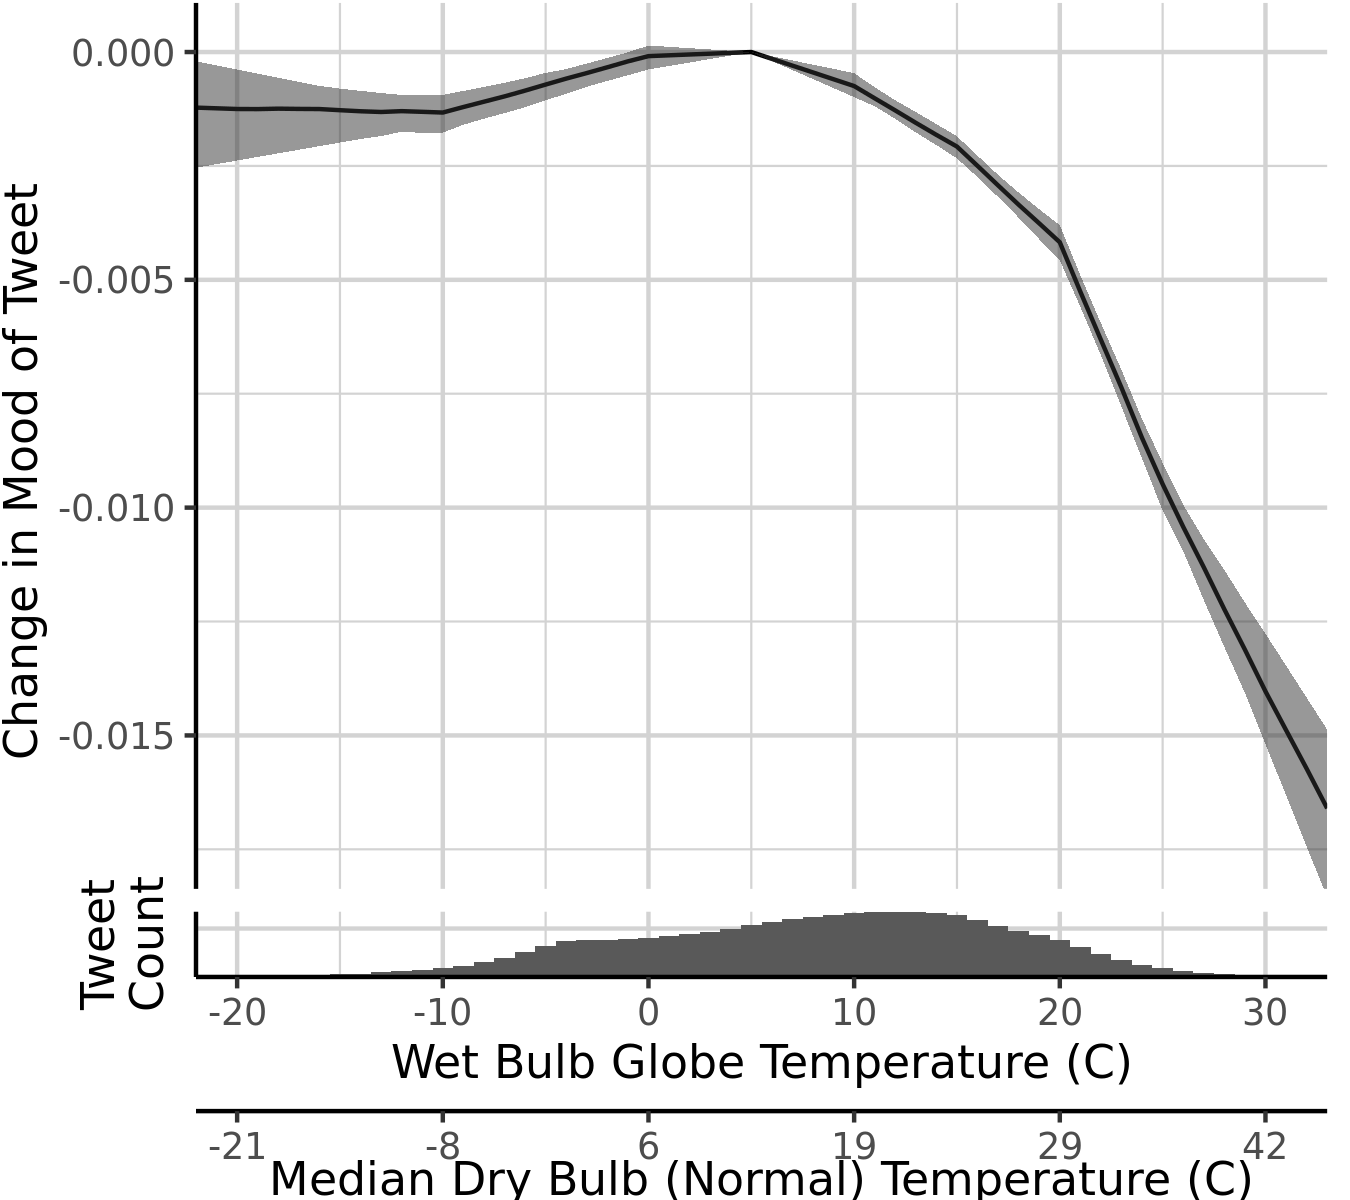
\includegraphics[width=0.5\linewidth]{../res/wbgt.png}
  \caption{Relationship between Wet Bulb Globe Temperature (WBGT) and sentiment in tweets.  As temperatures increase, sentiment declines.}
  \label{fig:wbgt-income}
\end{figure}

Sentiment is highest at a WBGT of 5 degrees celsius (a dry bulb temperature typically around 12C/54F).  The greatest declines in sentiment are observed between 20-25 degrees WBGT (dry bulb 29-36C/84-97F).  Sentiment also declines with colder temperatures, but only slightly.   

\begin{figure}[H]
\centering
\begin{subfigure}{.5\textwidth}
  \centering
  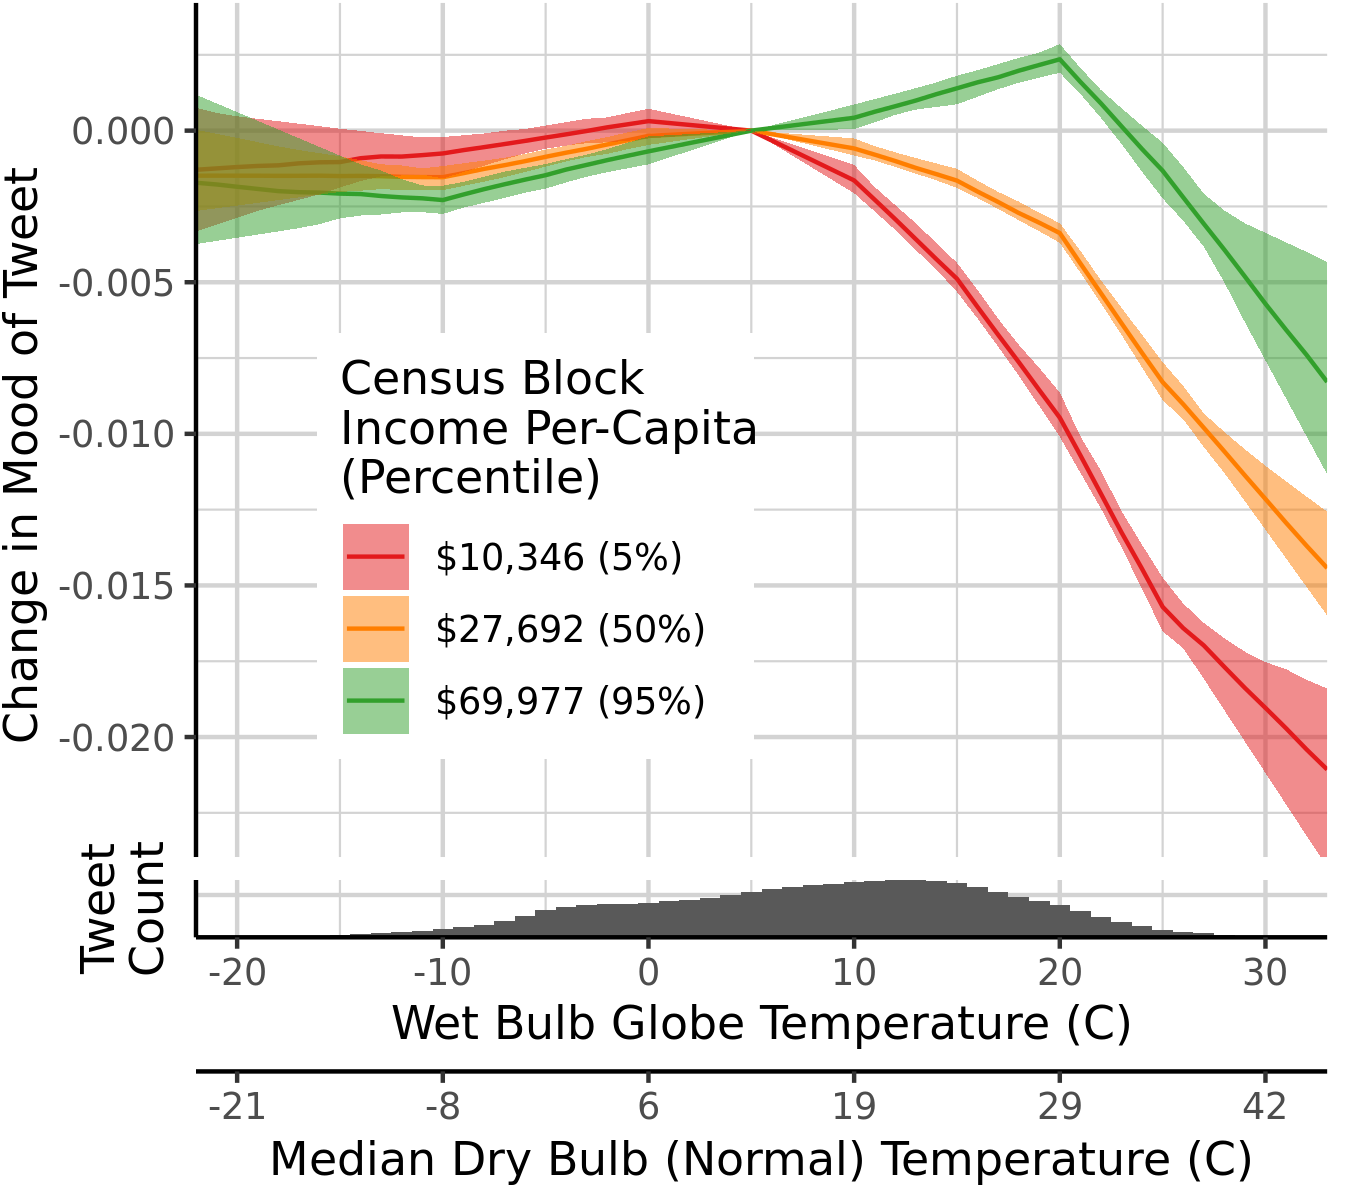
\includegraphics[width=\linewidth]{../res/wbgt-income.png}
  %\caption{WBGT-sentiment relationship as moderated by neighborhood income.}
  \label{fig:sub1}
\end{subfigure}%
\begin{subfigure}{.5\textwidth}
  \centering
  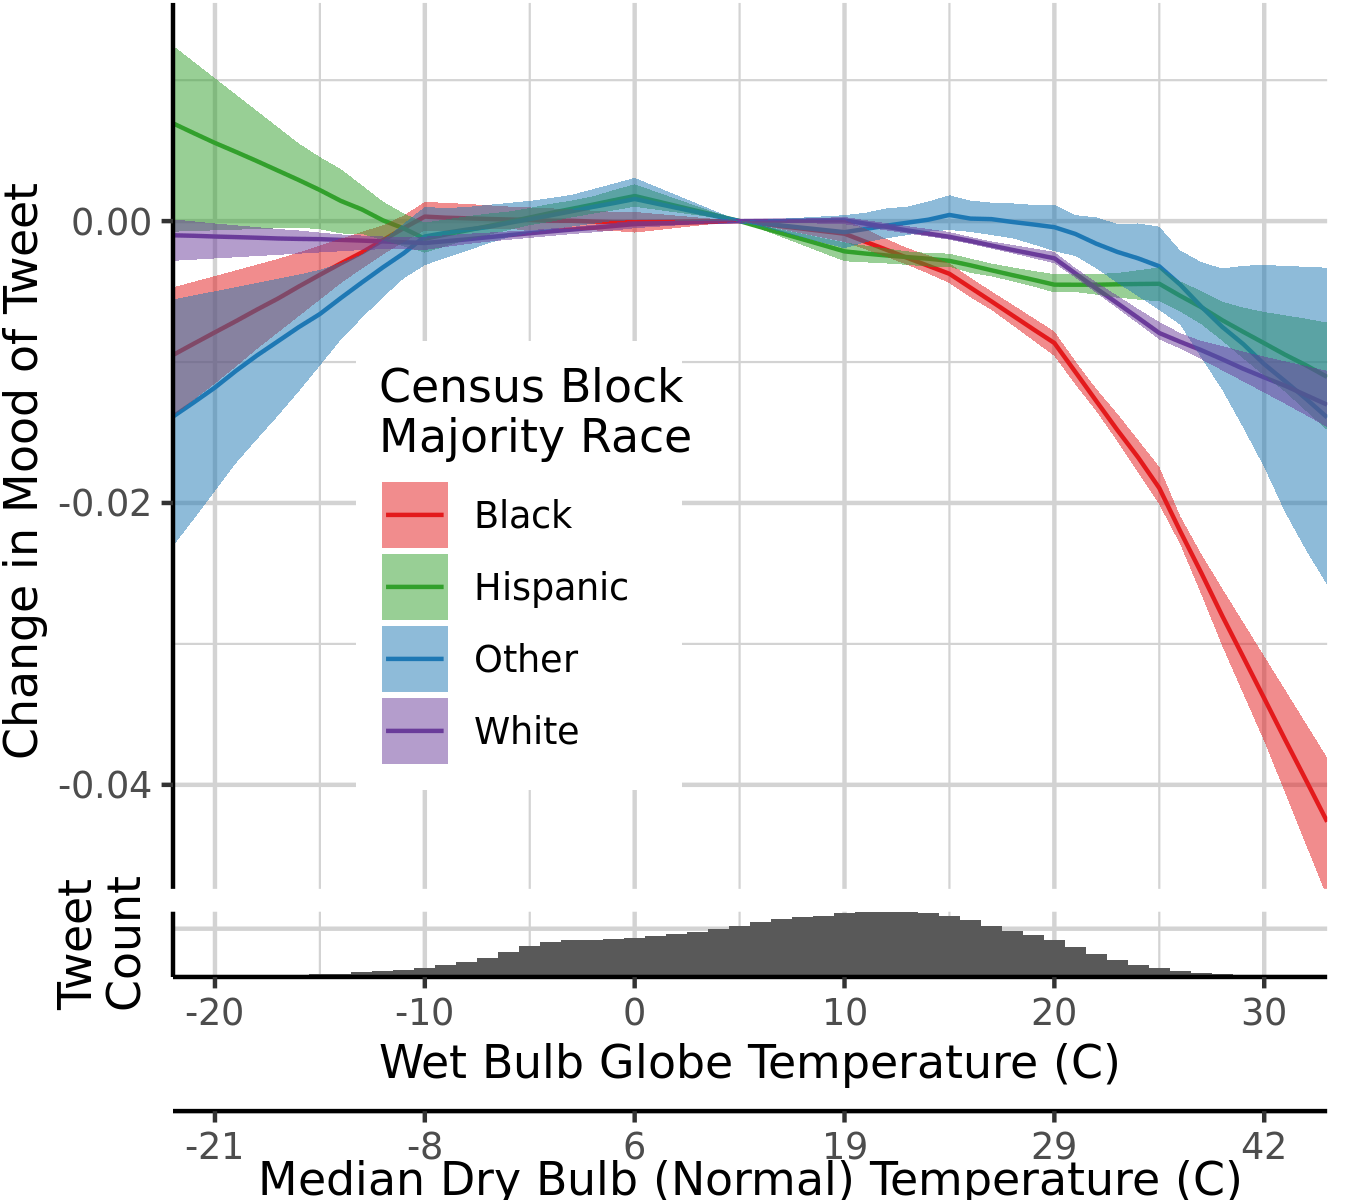
\includegraphics[width=\linewidth]{../res/wbgt-race_q.png}
  %\caption{WBGT-sentiment relationship as moderated by neighborhood majority race.}
  \label{fig:sub2}
\end{subfigure}
\caption{How the relationship between WBGT and sentiment is moderated }
\label{fig:test}
\end{figure}



\begin{figure}[H]
  \centering
  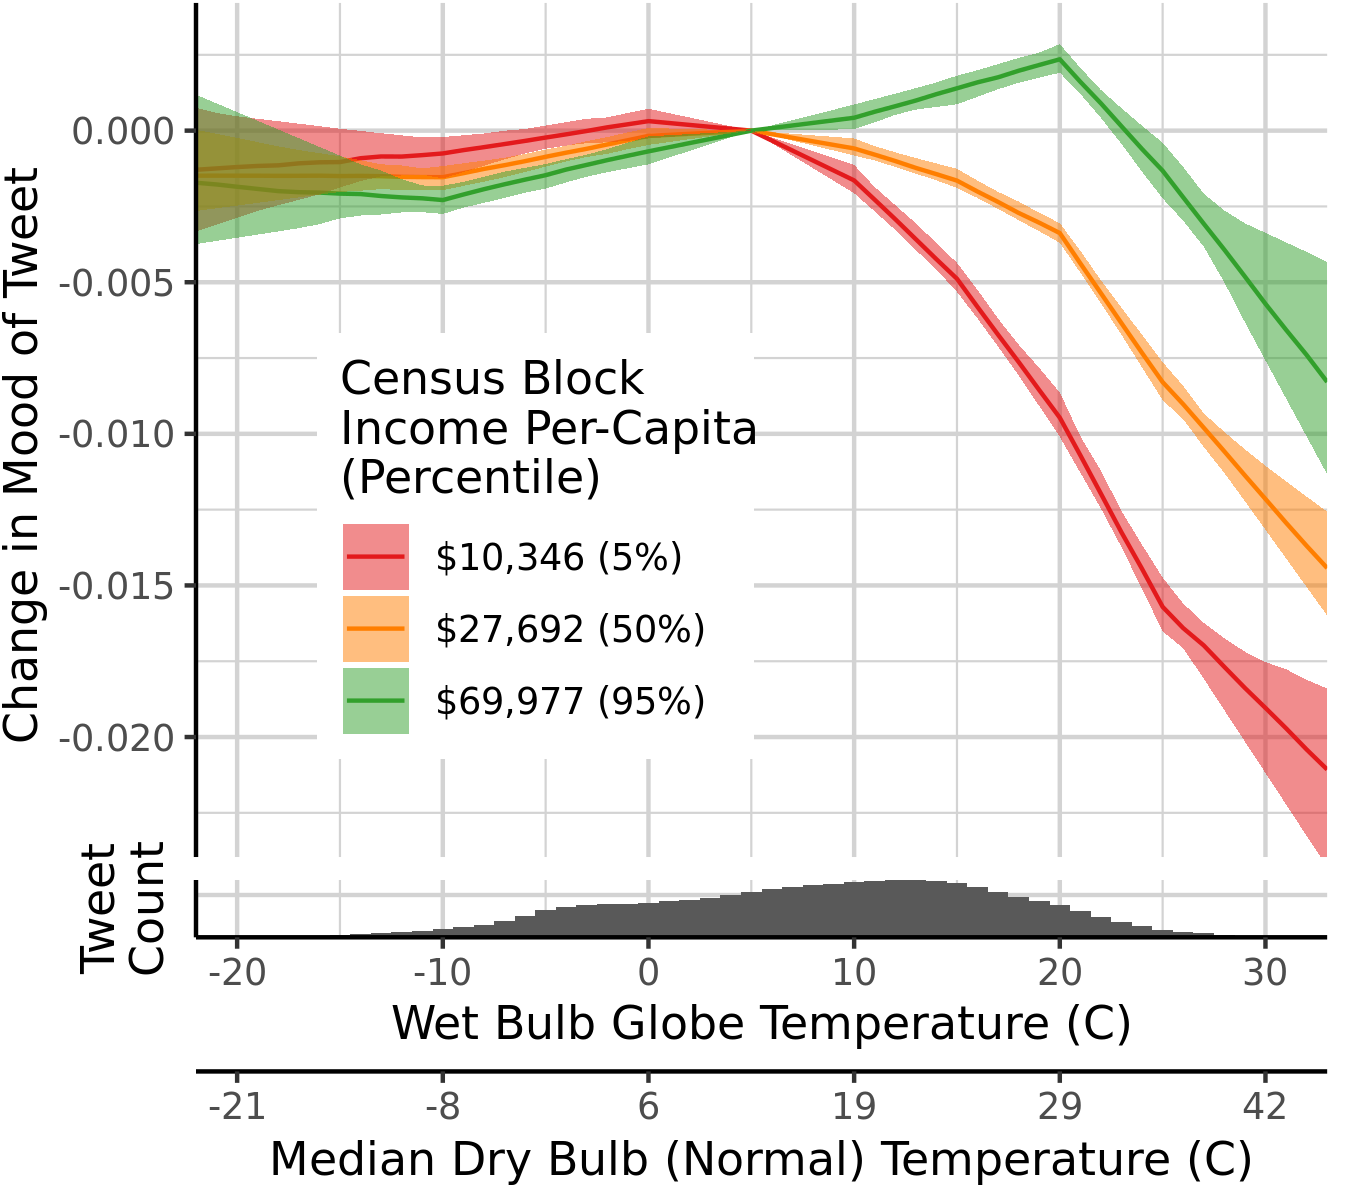
\includegraphics[width=\linewidth]{../res/wbgt-income.png}
  \caption{Change in sentiment across census block income groups as the Wet Bulb Globe Temperature increases.  For census blocks at the 5th percentile for income, even mild temperatures are associated with decreases in mood, while at higher temperatures, sentiment continues to decline.  For high-income census blocks at the 95th percentile, on the other hand, temperature must be quite high before a decrease in sentiment is observed.}
  \label{fig:wbgt-income}
\end{figure}


\begin{figure}[H]
  \centering
  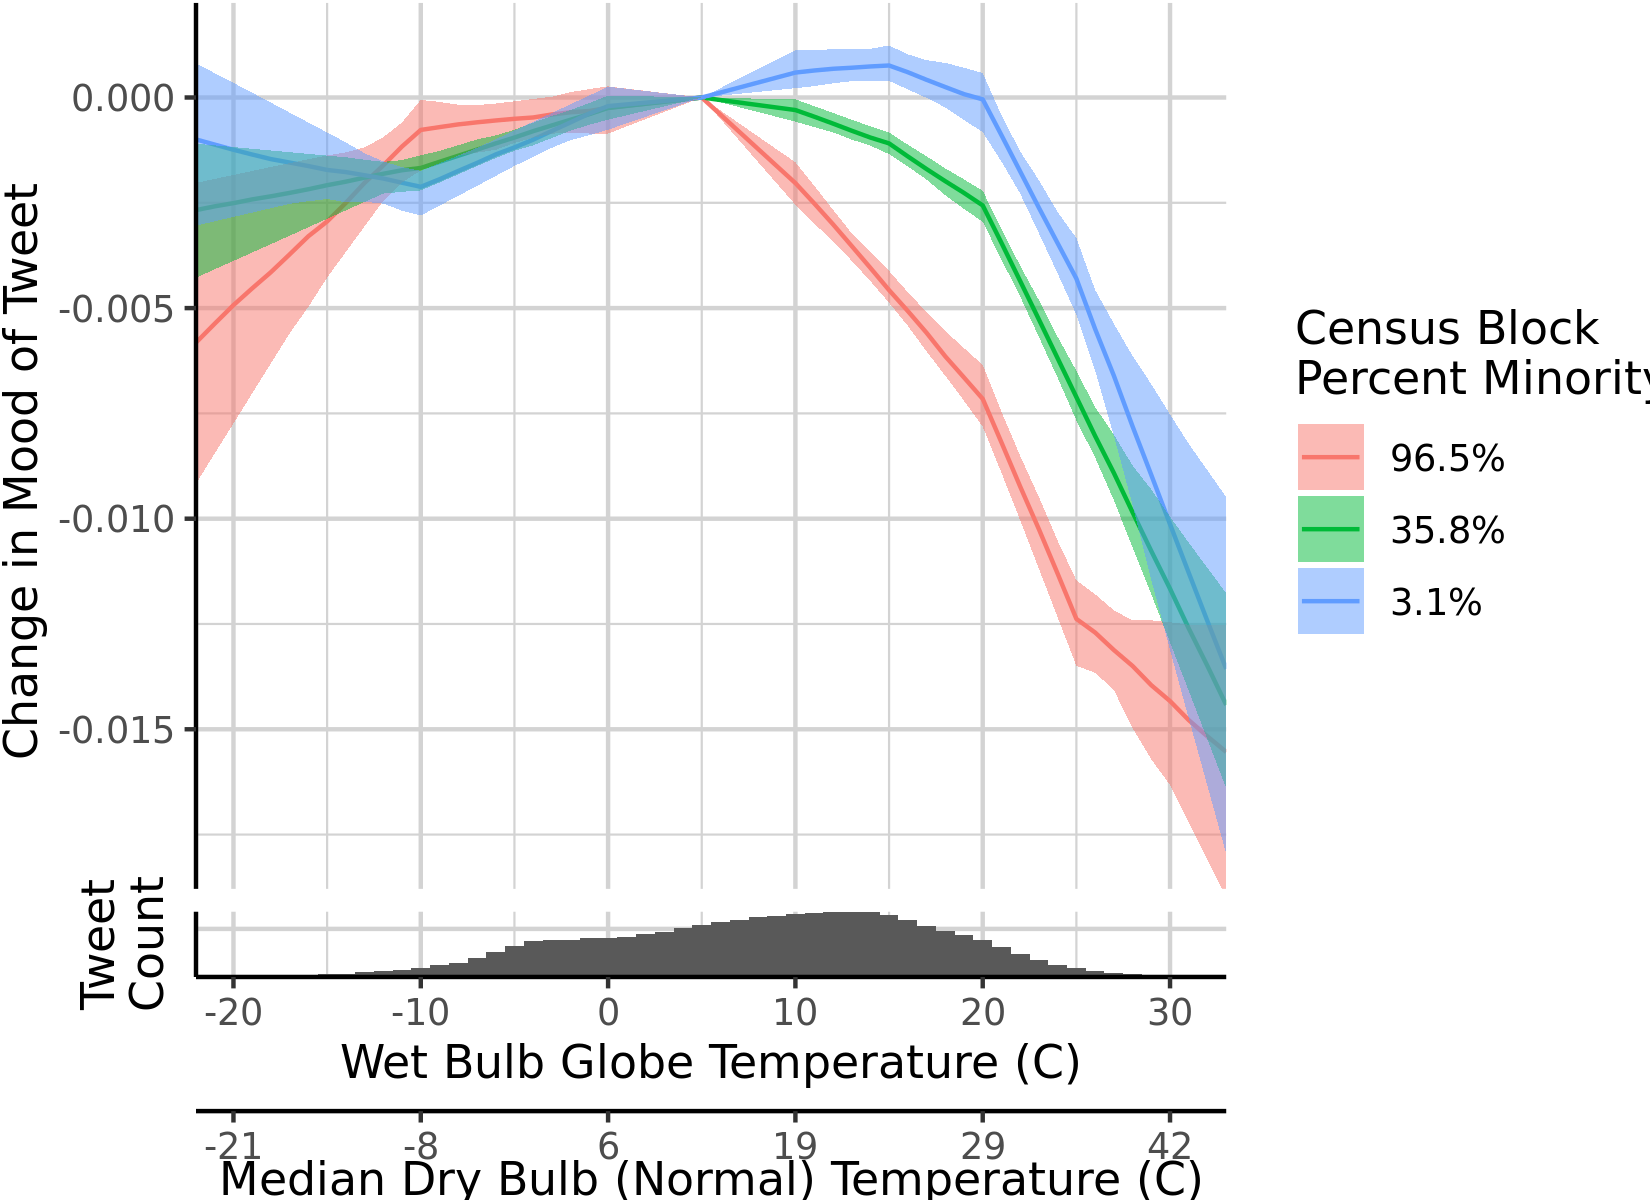
\includegraphics[width=\linewidth]{../res/wbgt-race.png}
  \caption{Change in sentiment across census block income groups as the Wet Bulb Globe Temperature increases.  For census blocks at the 5th percentile for income, even mild temperatures are associated with decreases in mood, while at higher temperatures, sentiment continues to decline.  For high-income census blocks at the 95th percentile, on the other hand, temperature must be quite high before a decrease in sentiment is observed.}
  \label{fig:wbgt-income}
\end{figure}



Figure of heatmap of tweet density across USA (pick a year? entire dataset of georeferenced tweets?)

(sub-section) TEMPERATURE and HUMIDITY
Figure of distribution of max and min temperatures
Comment from Patrick Baylis on our "preliminary results". 2nd comment from Patrick

(sub-section) INCOME

(sub-section?) SENTIMENT
Figure of distribution of observed sentiment scores (by Hedonometer, Vader, etc.)

Comment from Patrick Baylis on our "preliminary results" doc


\section{Discussion}

\section{Data}
A proposed list of tables and figures:
Figures for location of USA Tweets (to show aggregation and coverage).
Figures of income blocks and temperature extremes.
Table 1. Variable descriptions for what's included in our models.
Table 2. Descriptive statistics for datasets/variables we include.
Table 3. Model results with variables included in the models coefficients, SEs, p-values, sample size.
Appendix table. Sentiment scores across all types we considered.
\begin{figure}[H]
  \centering
  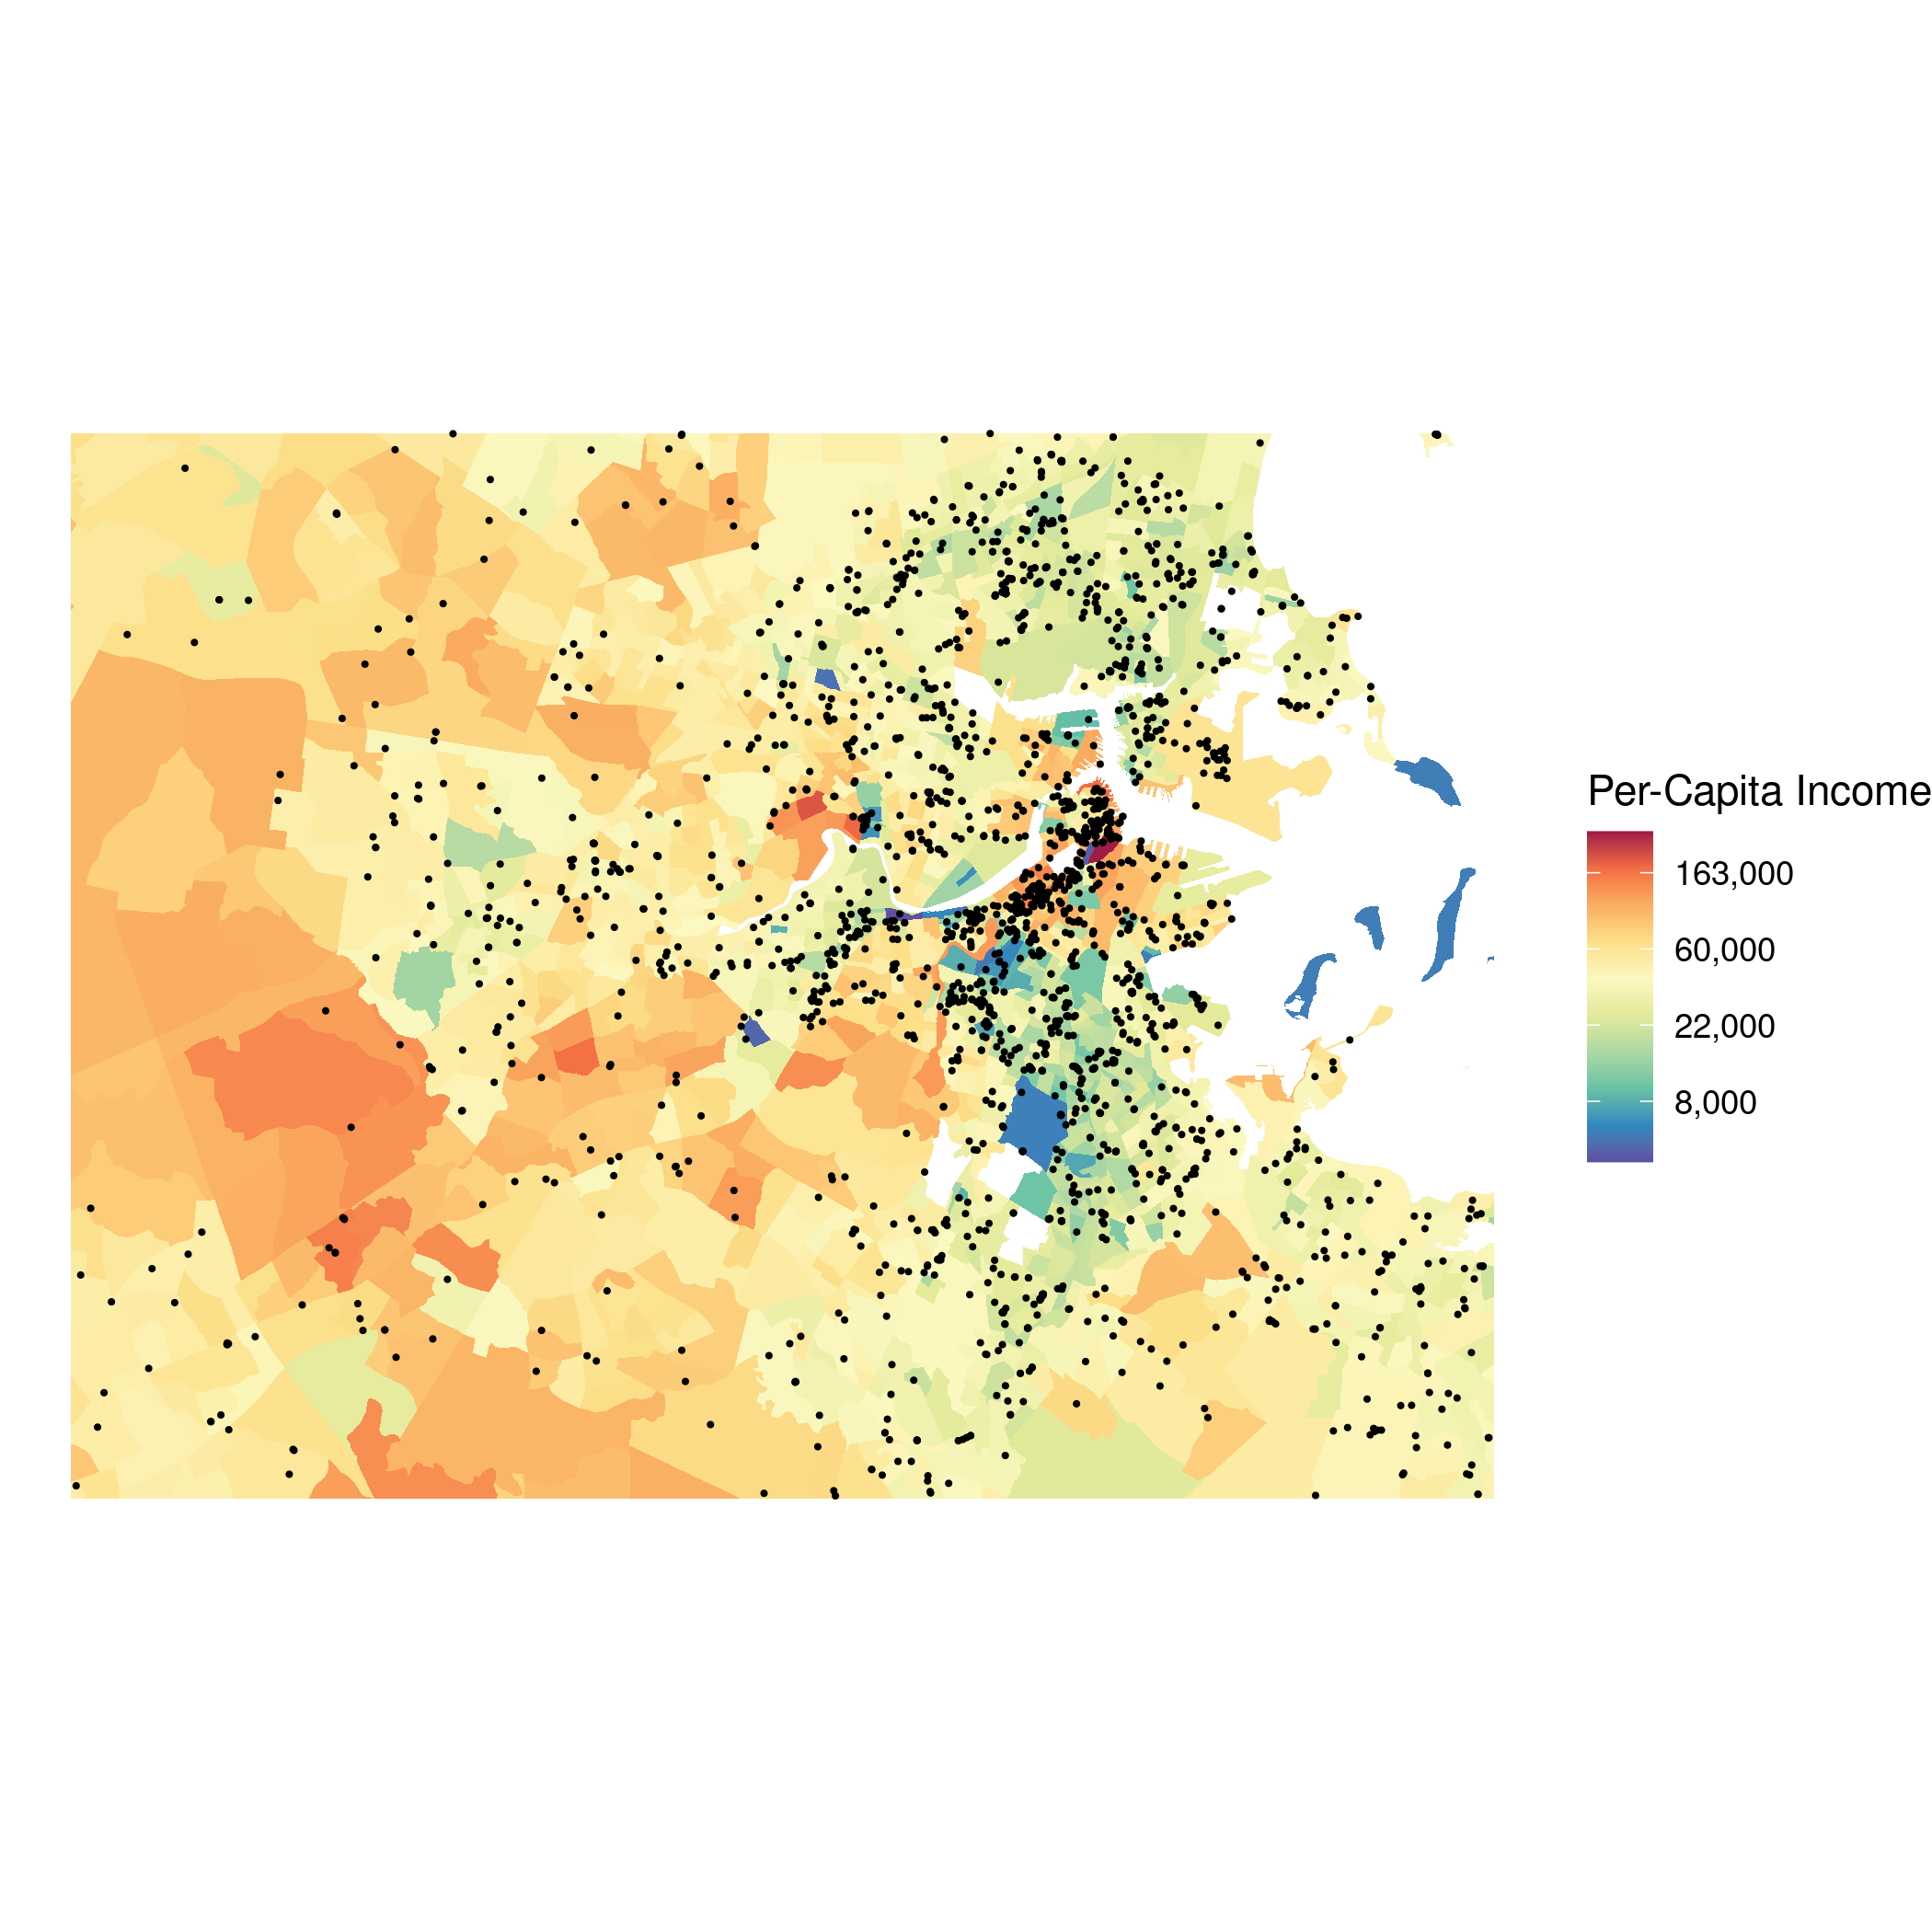
\includegraphics[width=\linewidth]{../res/Boston_Map.png}
  \caption{Here is a map of all tweets in boston, overlaid with income by census block}
  \label{fig:timeseries}
\end{figure}

\section{Methods}
\subsection{Tweets}
We used data from 243 million geolocated tweets from the lower 48 states from the years 2009 to 2019.  

Text data used for this project come from Twitter via the University of Vermont’s (UVM) agreement with Twitter to access its streaming API - colloquially referred to as the Decahose. The "decahose" provides public access to a random 10\% of all public messages on Twitter. The UVM special agreement with Twitter allows for access to this data for research and analysis purposes and we have complied with all the terms of service for Twitter and UVM. 
The Twitter data consists of publicly posted messages, or Tweets, that are short status messages users post to the platform. We used all geolocated Tweets from the Decahose for the period 2009-2019. We only considered users’ original content, thus did not include retweets in our analysis.

\subsection{Weather}
We used data on local weather conditions from the North American Land Data Assimilation System (NLDAS), a gridded product developed by several collaborative institutions, including NOAA, NASA, Princeton University, and the University of Washington.  This dataset is available at an hourly temporal resolution, and at 1/8th decimal degree spatial resolution, and integrates a large quantity of observation-based and modeled data  \cite{xia_continental-scale_2012}.  For the exact hour and location of each tweet, we extracted temperature, specific humidity, air pressure, total precipitation, shortwave radiation, and wind speed.  

Because metrics of apparent temperature that take into account humidity and other factors can better account for the impacts of heat stress on human health and wellbeing, we calculate the Wet Bulb Globe Temperature (WBGT) at the time and location of each tweet.  WBGT is the temperature that a wet globe thermometer would read in direct sunlight, and gives a reading lower than a dry bulb temperature would show due to evaporative cooling, and can be estimated given normal temperature, relative humidity, solar radiation, and wind speed.  Because evaporative cooling is how humans cool themselves through perspiration, this temperature better indicates the heat stress that people are experiencing.  Metrics like WBGT that account for the effects of humidity and other factors on heat stress have been associated with diminished economic output \cite{rao2020projections}, increased crime \cite{hu2017impact}, increased mortality \cite{chien2016spatiotemporal, armstrong2019role}, and worsened mental health outcomes \cite{vida2012relationship, ding2016importance}.

Using temperature, specific humidity, and pressure, we derived relative humidity using methods described by  \cite{bolton_computation_1980}.  We then calculated the WBGT using the formula described by \cite{heo2019comparison}.

\subsection{Socio-Econoimc Data}
We used data from the American Communit   Survey administered by the US Census to income levels and the racial composition of neighborhoods where tweets were located.  Data was at the level of the census block group, the smallest unit for which the census releases public data.

ACS data is released to cover five-year periods.  We therefore matched each tweet with census block group data from the year at the middle year of each survey's five-year range.  For example, tweets from 2014 were matched to data from the 2012-2016 ACS.  Because the most recent available data was from 2014-2018, all tweets from year years greater than 2016 were matched to this dataset.  Data was downloaded from the IPUMS NHGIS service provided by the University of Minnesota.

Mean annual income per capita is provided by the ACS, and we standardized this variable so that the values for each year were in 2019 dollars.  For racial categories, we combined the various categories provided by the ACS into four racial groups: non-Hispanic white, non-Hispanic black, Hispanic of any race, and an "other" category for non-Hispanic people who were neither black nor white, such as Asian, Native American, or mixed-race people.


\subsection{Sentiment}

WE EXCLUDED WEATHER TERMS

We assessed the sentiment expressed in text using several of the most commonly used measures of sentiment. Each of the measures uses validated dictionaries of words that have been assigned positive and negative scores and compares these words with words in the text corpora of interest. For measures of sentiment, we used the Hedonometer \href{https://hedonometer.org/timeseries/en_all/}{(link)}, Afinn \href{http://corpustext.com/reference/sentiment_afinn.html}{(link)}, Textblob \href{https://textblob.readthedocs.io/en/dev/}{(link)}, Vader , SentiwordNet and LIWC tools. These tools assign positive and negative scores to words, then average the scores for each text string. Our text data was multilingual, which can present challenges with analyzing text (cite). Given our interest only in the collection of words used (in aggregate) and not the sequence or nuance of the phrases, we translated all languages into English using Google Translate API and the Microsoft Azure API cognitive services (translator text API) before conducting the sentiment analyses.

Some papers we might cite in this section (only for multilingual work): Vilares et al. 2017 , Lo et al. 2017, Dashtipour et al. 2016.

Discuss issues with text data (gtp) - that it doesn’t capture emoticons, code switching (e.g., [good job! \#fail]), etc.

Issues with sample population (non-representative)

Issues with what people say on social media being attenuated or mismatched from actual emotional state

\subsubsection{Hedonometer}
The Hedonometer \cite{dodds_temporal_2011} is a corpus-based technique to get sentiment score from multi-lingual texts. The core steps are (1) building human evaluations of the happiness of a set of individual words, and (2)using a naive algorithm for scaling up from individual words to texts. For the English corpus, Dodds and others \cite{dodds_temporal_2011} collect 10,222 unique words and used crowd-sourcing platform Amazon Mechanical Turk to get human evaluation of happiness degree for each word in an integer scale from 1 to 9, representing a sad to happy spectrum. Score 5 represents neutral words. Each word will be calculated average score and then the word and happiness score are compiled into a dataset (labMT 1.0). Some illustrative example of words are: 

\[h_{avg} (\text{laughter}) = 8.50 \]
\[h_{avg} (\text{the}) = 4.98\]
\[h_{avg} (\text{hate}) = 2.34\]

The sentiment score for single text will be the mean happiness score for all words in the text.


\subsubsection{VADER}
The VADER sentiment corpus was proposed by Gilbert and Hutto \cite{gilbert_vader_2014} and stands for 'Valence Aware Dictionary for sentiment Reasoning'. It is is a lexicon and rule-based sentiment analysis tool that is specifically attuned to sentiments expressed in social media by incorporating lexical features common to sentiment expression in microblogs

\subsection{Modeling}
We assessed how expressed sentiment is affect by three weather variables: wet bulb globe temperature, precipitation, and sunshine.  Moreover, we modeled how neighborhood income affects the relationship between these weather variables and sentiment.

Our model takes the following form:
\begin{equation}
    y = \beta_0 + f_t(t) + f_{mt}(m t) + \beta_p p + \beta_{mp} m s + \beta_s s + \beta_{ms} m s + \Phi + \epsilon
\end{equation}

Where $y$ is the sentiment of a tweet, $t$ is the wet bulb globe temperature at the hour of the tweet, $p$ is a binary variable indicating whether it rained at the hour of the tweet, $s$ is the income shortwave radiation, or sunshine, in $W/m^2$, at the hour of the tweet, and $m$ is the log-transformed average income in the census block where the tweet originated.  We estimate the 


STANDARD ERRORS


\subsection{Data Processing}
We analyzed meteorological data using the R statistics open-source program version 3.6.2  (R Core Team 2019) using R Studio version 1.2.1335 (RStudio Team, 2019) and the raster \href{https://www.rdocumentation.org/packages/raster/versions/3.3-13}{(link)}, sp \href{https://cran.r-project.org/web/packages/sp/index.html}{(link)}, sf \href{https://cran.r-project.org/web/packages/sf/index.html}{(link)}, and stars \href{https://cran.r-project.org/web/packages/stars/index.html}{(link)} processing and geospatial packages installed. We analyized sentiment data using python version x.x.x with pandas \href{https://pandas.pydata.org/}{(link)} and numpy \href{https://numpy.org/}{(link)} packages installed. We extracted meteorological data using the geolocated coordinates from the Twitter posts (latitude and longitude). We calculated mean climatological scores (z-scores)using baseline meteorological data from 1990 to present, calculated at a quarter degree resolution, and based on the long-term averages and standard deviation. We calculated z-scores for each day and the overall annual average z-score. For text data cleaning we used the python package tweet-preprocessor \href{https://pypi.org/project/tweet-preprocessor/}{(link)} to remove all text and characters not part of the main text phrase (e.g., URLs, mentions, GIFs, etc.). We converted all dates and times to UTC format.

[NEED SOME TEXT ABOUT GOOGLE EARTH ENGINE AND MICROSOFT AI FOR EARTH] We conducted all data analyses on Microsoft AI for Earth's online cloud-computing environment using a combination of existing data analysis packages and scripts we developed. We used GitHub as a repository for all scripts we used in this project (link to the Git repo). To run ABC analysis, we used Microsoft's CBA package. To run XYZ analysis, we used Microsoft's ZYX package. 

%%KEY POINTS TO DISCUSS

% Link between twitter mood and other very bad outcomes (crime, suicide)

% Baselines: this could also be interpreted as: poor are less affected by the cold\textbf{:}

% Caveats:
    % Uncertainties from census blocks (low income, young areas).  This is why we used a linaer effect instead of a binned effect.
    % We cant speak to types of mental heath that are worsening - depression, anxiety, and post-traumatic stress, etc.  Just a general overview

\section{Conclusion}

\section{Acknowledgements}
For funding, advising, SESYNC grant number?, etc.
This work was supported by the National Socio-Environmental Synthesis Center (SESYNC) under funding received from the National Science Foundation DBI-1639145.

\printbibliography

\section*{Supplemental Info}
\setcounter{table}{0}
\setcounter{figure}{0}
\setcounter{section}{0}
\renewcommand{\thetable}{S\arabic{table}}
\renewcommand{\thefigure}{S\arabic{figure}}
\renewcommand{\thesection}{S\arabic{section}}

\subsection{Other Sentiment Metrics}

\subsection{Precipitation}


%Supplement will have:

%Equations used for RH and WBGT


% Robustness checks:

    % Other sentiment metrics
    
    % 




%%%%%%%%%%%%%%%%%%%%%%%%%%%%%%%%%%%%%%%%%%%%%%%%
% Paste Bin
%%%%%%%%%%%%%%%%%%%%%%%%%%%%%%%%%%%%%%%%%%%%%%%%%%

\subsection{Land Cover}
To estimate land cover categories and the percentage of tree cover and impervious surfaces, we used data from the National Land Cover Database (NLCD) from the USGS' 2011  \cite{homer_completion_2015} and 2016 \cite{yang_new_2018} landcover datasets. These datasets are national land cover dataset prepared by the Multi-Resolution Land Characteristics (MRLC) Consortium.  These data are at the thirty meter resolution, and provide estimates of the fraction of tree cover and impervious surfaces.  We then associated each tweet with the land cover fraction for the nearest available year and pixel using the geolocation associated with each tweet, extracting landcover values from whichever land cover dataset year was closest in time to the date timestamp of each tweet. We used tree cover as a proxy for amount of potential shade and heat relief in a particular area and can be broadly indicative of generalized wealth. We use impervious surface cover as a proxy for relative proximity to potential natural shade and heat relief, and because individuals in urban environments may be exposed to the urban heat island effect. [NEED SOME CITATIONS HERE] 

\section*{Text Snippets Not Used Here but We Might Want to Keep}
Gaps on above we intend to fill in:
Our research aim and objectives
Its contribution

From Intro/Background
Changes in climate result in fluctuations in the frequency, intensity, spatial extent, duration, and timing of weather resulting in unprecedented climate extremes . Changing climate is putting pressures on environmental and social system health and necessitating changes in how we respond to environmental conditions and anticipate (and plan for) future conditions. (cite IPCC report on health and environment, also cite the Lancet report on climate and health). 

[from our Jan/Feb 2020 draft working manuscript in Google Docs]
Climate change is a universal issue as it affects every country in the world. Changes in climate result in fluctuations in the frequency, intensity, spatial extent, duration, and timing of weather resulting in unprecedented climate extremes \href{https://www.ipcc.ch/site/assets/uploads/2018/03/SREX-Chap3_FINAL-1.pdf}{(link)}. Changing climate is putting pressures on environmental and social system health and necessitating changes in how we respond to environmental conditions and anticipate (and plan for) future conditions. (cite IPCC report on health and environment, also cite the Lancet report on climate and health).

Dehghan et al. 2012  The evaluation of heat stress through monitoring environmental factors and physiological responses in melting and casting industries workers. High prevalence of industrial workers experiencing heat stress. Relatively low humidity conditions made it necessary to alter their work/rest cycles. \href{http://www.ijehe.org/article.asp?issn=2277-9183;year=2012;volume=1;issue=1;spage=21;epage=21;aulast=Dehghan}{link}

?. (from intro) Increased variability around environmental norms (e.g., lower/higher temperatures, changes in timing, magnitude, duration of precipitation or dry spells, etc.) can amplify the effects on systems. Increased uncertainty in planning for these events and ability to respond to them (adaptive capacity). - draw in cultural risk and social practice theories, here?

NOTES: Scaling back out → we are exploring temperature and sentiment (in Tweets) across languages. This is a clear innovation that builds on the existing work from the Baylis et al. team (in their plosONE paper) and in fact is something they recommended be done - recommended to us as a team, too.

We know that temps affect sentiment, but (1) Is this effect observable across languages? (2) Is this effect moderated by factors like wealth?

We could ask similar questions substituting in the patent filings, too (sub-project 3 in our previous work-plan). These questions - and likely the methods used to answer these questions - are quite portable and compelling and may take the form for the patent work like this: Given we know that temperature affects worker productivity (increased temp increases productivity up to 13C, sharp negative decline thereafter), can we observe this pattern in patent filings? Across various geographies? Are there lags in filings after unusually cold or hot temperature events?

For the Twitter data, using text translated into a base language is fully appropriate and a frequently used method if looking for latent text structures in topic modeling (see Proksch et al. 2018 for an alternative). For sentiment analysis on multilingual datasets, we'll need to decide on an approach (see Ling Lo et al. 2016 review) but there are several that are good. If we wanted to use another open-source option, we could follow that laid out by Lucas and others (2015).

Proskch et al. 2018 paper --> \href{https://onlinelibrary.wiley.com/doi/full/10.1111/lsq.12218}{link} 

Ling Lo et al. 2016 paper --> \href{https://link.springer.com/article/10.1007/s10462-016-9508-4}{link} 

Lucas et al. 2015 paper --> \href{https://www.cambridge.org/core/journals/political-analysis/article/computerassisted-text-analysis-for-comparative-politics/CC8B2CF63A8CC36FE00A13F9839F92BB}{link}
 





\end{document}
